\documentclass[10pt]{beamer}

\usepackage[T2A]{fontenc}
\usepackage[utf8]{inputenc}
\usepackage[russian,english]{babel}

\usefonttheme[onlymath]{serif}

\usetheme[progressbar=frametitle]{metropolis}
\usepackage{appendixnumberbeamer}

\usepackage{booktabs}
\usepackage[scale=2]{ccicons}

\usepackage{pgfplots}
\usepgfplotslibrary{dateplot}

\usepackage{xspace}
\newcommand{\themename}{\textbf{\textsc{metropolis}}\xspace}
\newcommand{\TODO}[1]{\textbf{\textcolor{red}{TODO: #1}}}

\date{}
\author{Екатерина Тузова}

\usepackage{mathrsfs}

\title{Лекция 4}
\subtitle{Деревья принятия решений}

\begin{document}

\maketitle

\section{Разбор летучки}

\section{Мотивирующий пример}
{\foot{\href{https://www.kaggle.com/alopez247/pokemon}{Pokémon for Data Mining and Machine Learning (https://www.kaggle.com/alopez247/pokemon)}}
\begin{frame}{Мотивирующий пример}
	\begin{figure}
	    \centering
	    \subfloat{{
\includegraphics[width=2cm]{../lecture2/images/Bulbasaur} }}
	    \qquad
	    \subfloat{{
\includegraphics[width=2cm]{../lecture2/images/Mewtwo} }}
    	    \qquad
    	    \subfloat{{
\includegraphics[width=2cm]{../lecture2/images/Volcanion} }}
    	    \qquad
    	    \subfloat{{
\includegraphics[width=2cm]{../lecture2/images/Ekans} }}
    	    \qquad
    	    \subfloat{{
\includegraphics[width=2cm]{../lecture2/images/Nidorina} }}
	    \qquad 
    	    \subfloat{{
\includegraphics[width=2cm]{../lecture2/images/Rattata} }}
	    \qquad
    	    \subfloat{{
\includegraphics[width=2cm]{../lecture2/images/Sandshrew} }}
	    \qquad
    	    \subfloat{{
\includegraphics[width=2cm]{../lecture2/images/Articuno} }}    	        	    
	\end{figure}
\end{frame}
}

\begin{frame}{Датасет}
  \centering
	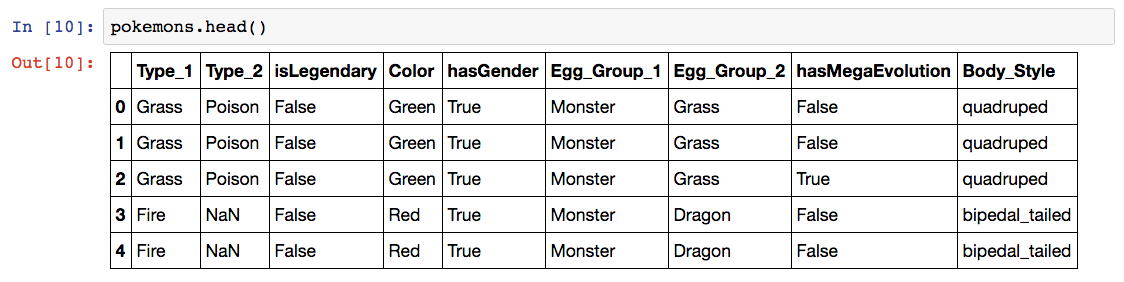
\includegraphics[width=\textwidth]{images/pokemons}
\end{frame}

\begin{frame}{Мотивация}
  \begin{center}
	  
\includegraphics[width=\textwidth, height=0.8 \textheight, keepaspectratio]{images/distance}
	  \end{center}
\end{frame}

\begin{frame}{Логические закономерности}
	${X^l = \left( x_i, y_i \right)_{i=1}^l}$ - обучающая выборка.\\
	\bigbreak
	\alert{Логическая закономерность} -- предикат ${\beta: X \rightarrow \left\{ 0, 1 \right\} }$, который удовлетворяет двум требованиям:\\
	\pause
	\begin{enumerate} 
		\item Интерпретируемость
		\pause
		\item Информативность относительно одного из классов ${c \in Y}$
	\end{enumerate}
\end{frame}

\begin{frame}{Логические закономерности}
	${X^l = \left( x_i, y_i \right)_{i=1}^l}$ -- обучающая выборка.\\
	\bigbreak
  Предикат ${\beta: X \rightarrow \left\{ 0, 1 \right\} }$\\
	\bigbreak
	\alert{Задача}: Найти множество логических закономерностей $\mathscr{B}$ по $X^l$.\\
	Построить алгоритм $a(X, \mathscr{B}) \rightarrow y$, способный классифицировать произвольный объект ${x \in X}$.
\end{frame}

\begin{frame}{Интерпретируемость}
	\begin{enumerate}
		\item Записывается на естественном языке
		\item Зависит от небольшого числа признаков
	\end{enumerate}
\end{frame}

\begin{frame}{Интерпретируемость}
  \centering
	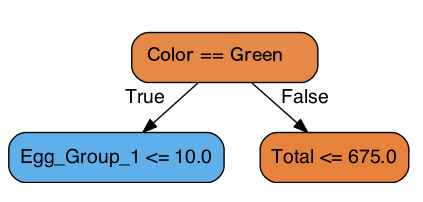
\includegraphics[width=\textwidth, height=0.8 \textheight, keepaspectratio]{images/beta1}
\end{frame}

\begin{frame}{Информативность}
  \alert{Идея}: Максимизировать количество правильно распознанных объектов класса $c$ и при этом минимизировать количество объектов, ошибочно классифицированных как класс $c$
  \pause
	\bigbreak
	$${ tp(\beta) = \# \left\{ x_i: \beta(x_i) = 1 , y_i = c \right\} \rightarrow \max }$$\\
	\pause
  \bigbreak
	$${ fp(\beta) = \# \left\{ x_i: \beta(x_i) = 1 , y_i \neq c \right\} \rightarrow \min }$$\\		
\end{frame}

\begin{frame}{Основные вопросы}
	\begin{enumerate}
		\item Какого вида закономерности $\beta(x)$ нужны?
		\item Как определять информативность? 
		\item Как выбирать закономерности?
		\item Как объединять закономерности в алгоритм?
	\end{enumerate}
\end{frame}

\section{Виды правил}

\begin{frame}{Виды правил}
	\begin{itemize} [<+->]
	\item[--] Пороговое условие\\
	$\beta(x) = \left[x^j \leq a_j \right]$ или  $\left[a_j \leq x^j \leq b_j \right]$
	\item[--] Конъюнкция из $J$ пороговых условий \\
	$\beta(x) = \bigwedge\limits_{j \in J} \left[a_j \leq x^j \leq b_j \right]$
	\item[--] Синдром -- выполнение не менее $d$ условий из $J$
	$\beta(x) = \left[\sum\limits_{j \in J} \left[a_j \leq x^j \leq b_j \right] \geq d \right]$
	\end{itemize}
\end{frame}

\section{Как собрать классификатор из закономерностей?}

\begin{frame}{Решающий список}
	\alert{Идея}:\\
	Возьмем $\beta_1(x), \beta_2(x), \dots, \beta_T(x)$ закономерностей и будем по порядку применять на объекте. 
	Как только предикат $\beta_i$ сработал -- вернем соответствующий класс $c_i$.\\
	\bigbreak
	\pause
	Каждое правило принимает окончательное решение $\Rightarrow$ ошибка правила равна ошибке всего алгоритма
\end{frame}

\begin{frame}{Бинарное решающее дерево}
	Бинарное решающее дерево -- алгоритм классификации $a(x, \beta)$, задающийся бинарным деревом:\\
	\begin{enumerate}[--]
	\item $\forall v \in V_{inner} \rightarrow \beta_v: X \rightarrow \left\{ 0,1\right\}$, $\beta \in \mathscr{B}$
	\item $\forall v \in V_{leaf} \rightarrow $ имя класса $c_v \in Y$\\
	
	\begin{figure}[htbp]
	  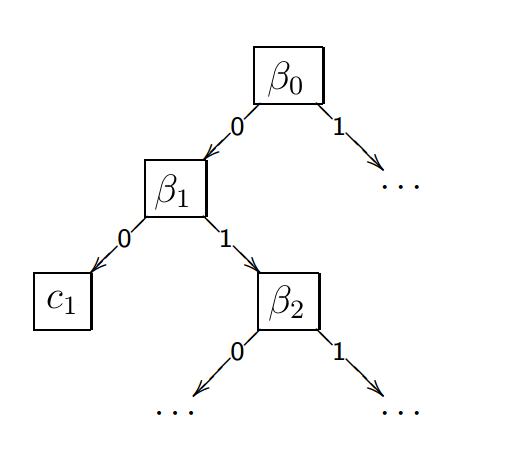
\includegraphics[height=150pt, keepaspectratio = true]{images/binary_tree}   
	\end{figure}
	\end{enumerate}
\end{frame}

\begin{frame}{Пример решающего дерева}
	  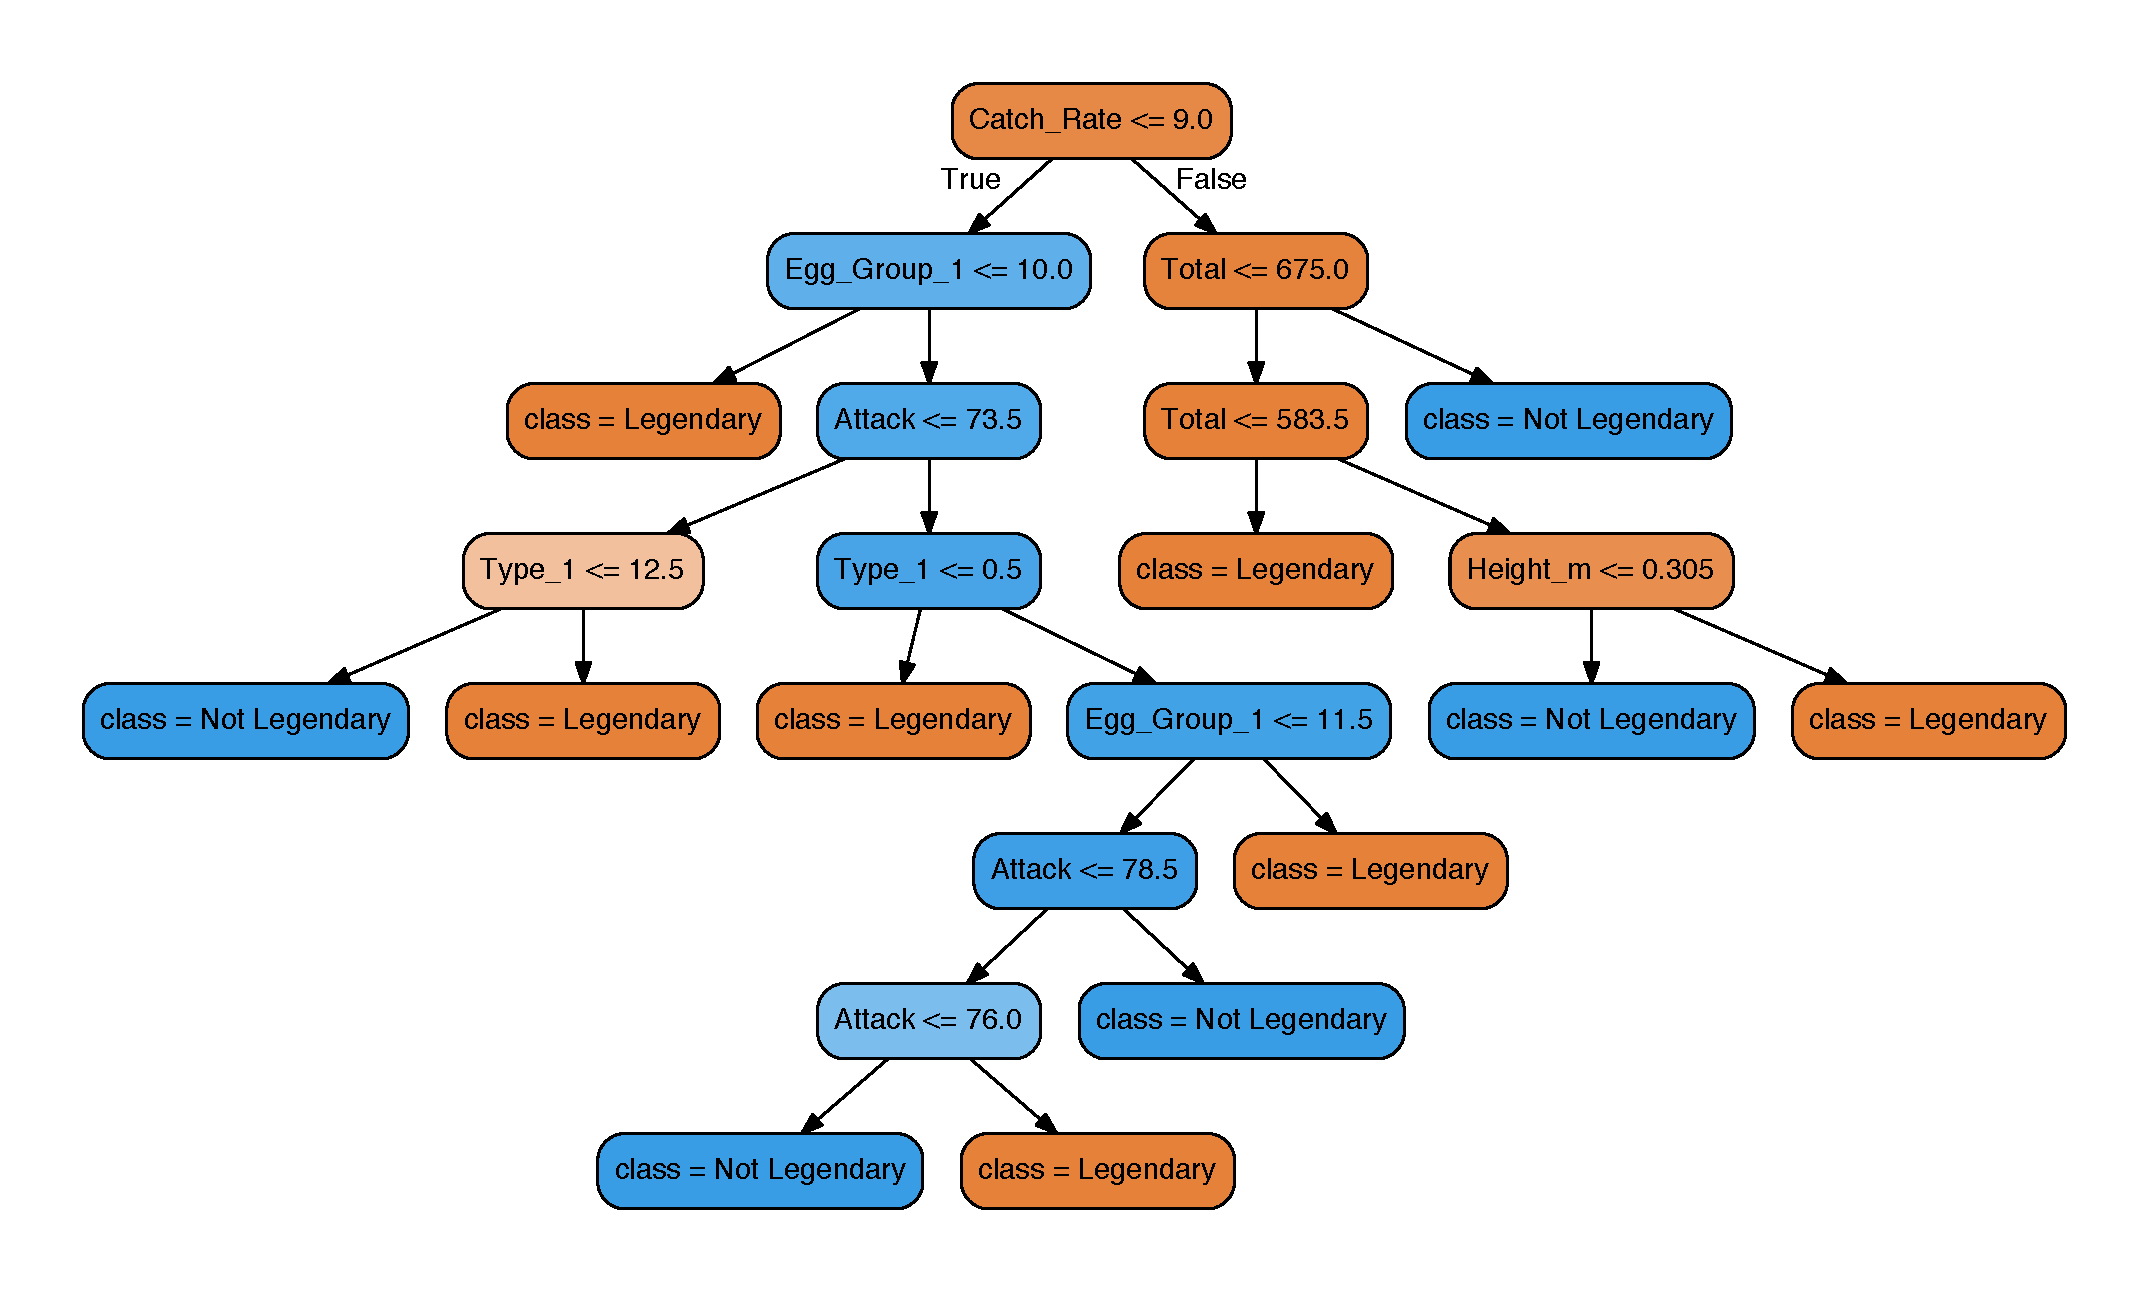
\includegraphics[height=\textheight, width=\textwidth, keepaspectratio = true]{images/pokemons-tree}   
\end{frame}

{\foot{Iterative Dichotomizer 3}
\begin{frame}{Алгоритм построения ID3}
  \begin{algorithmic}[1]
    \Function{LearnID3}{$U$, $\mathscr{B}$}
       \If {все объекты из $U$ лежат в одном классе $c \in Y$}
         \State \Return {новый лист $v$, $c_v = c$}
       \EndIf
       \State $\beta^* = \max\limits_{\beta \in \mathscr{B}} I(\beta, U)$
       \State $U_{left} = \left\{ x \in U : \beta^*(x) = 0\right\}$	
       \State $U_{right} = \left\{ x \in U : \beta^*(x) = 1\right\}$	
       \If {$U_{left} = \oslash$ или $U_{right} = \oslash$}
         \State \Return {$v$, $c_v$ = Majority($U$)}
       \EndIf
       \State Создать новую внутреннюю вершину $v$: $\beta_v = \beta^*$
       \State $L_v =$ LearnID3 ($U_{left}$, $\mathscr{B}$)
       \State $R_v =$ LearnID3 ($U_{right}$, $\mathscr{B}$)
       \State \Return $v$
    \EndFunction
  \end{algorithmic}    
\end{frame}
}

\section{Критерии информативности}

\begin{frame}{Оценивание информативности}
	${ tp(\beta) = \# \left\{ x_i: \beta(x_i) = 1 , y_i = c \right\} \rightarrow \max  }$ \\
  ${ tn(\beta) = \# \left\{ x_i: \beta(x_i) = 0 , y_i \neq c \right\} \rightarrow \max  }$ \\
	${ fp(\beta) = \# \left\{ x_i: \beta(x_i) = 1 , y_i \neq c \right\} \rightarrow \min}$ \\
	${ fn(\beta) = \# \left\{ x_i: \beta(x_i) = 0 , y_i = c \right\} \rightarrow \min}$ \\
	\bigbreak
	\pause
	$Precision = \frac{tp}{tp+fp}$\\
  $Recall = TPR = \frac{tp}{tp + fn}$\\
  $FPR = \frac{fp}{fp+tn}$\\
\end{frame}

\begin{frame}{Precision-Recall}
	\centering
	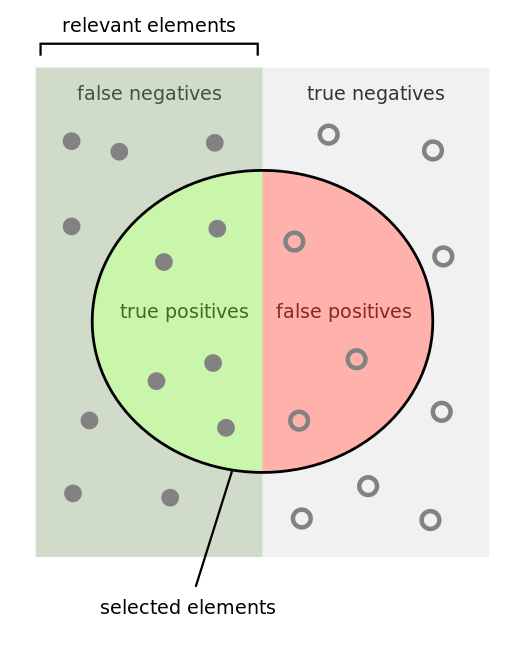
\includegraphics[width=\textwidth, height=0.9 \textheight, keepaspectratio]{images/precisionrecall}
\end{frame}

{\foot{ Receiver-operating characteristic}
\begin{frame}{ROC-кривая}
  \centering
  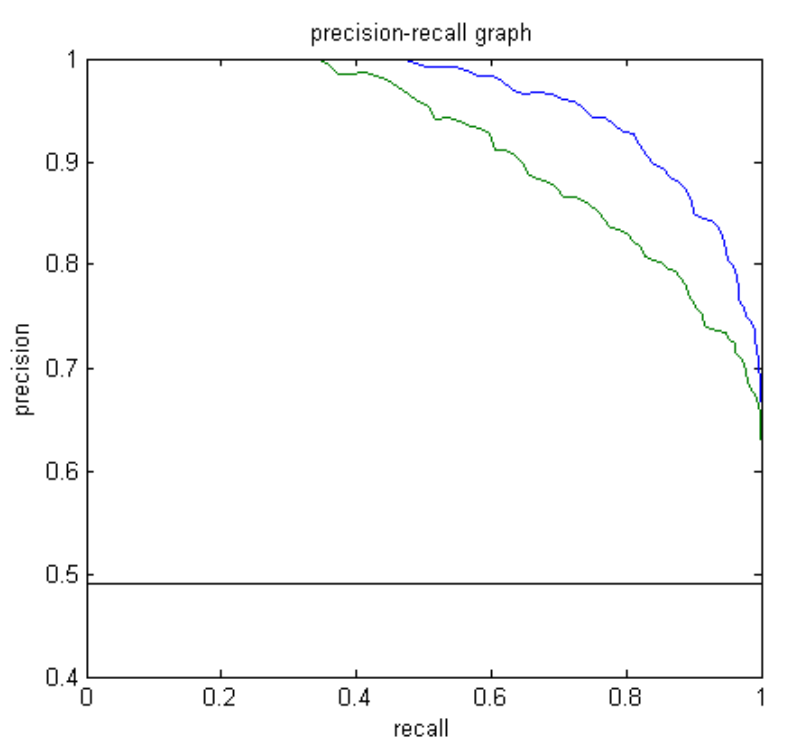
\includegraphics[height=0.7 \textheight, keepaspectratio = true]{images/roc}   \\
  AUC -- Area under the ROC curve
\end{frame}
}

\begin{frame}{Пример свертки двух критериев}
	Пусть число примеров искомого класса 200 и число остальных объектов 100\\
	\bigbreak
	\begin{tabular}{|r l|l|l|l|}
	  \hline 
	  $tp$ & $fp$ & $tp-fp$ & $tp-5fp$ & $Precision$\\ 
	  \hline \hline
	  50 & 0 & \textcolor{red}{50} & 50 & 1\\
	  \hline
	  100 & 50 & \textcolor{red}{50} & -150 & 0.6\\
	  \hline \hline
	  50 & 9 & 41 & \textcolor{red}{5} & \textcolor{red}{0.84}\\
	  \hline  
	  5 & 0 & 5 & \textcolor{red}{5} & \textcolor{red}{1}\\  
	  \hline 
	\end{tabular}
\end{frame}

\begin{frame}{Критерий Джини}
  $$I(\beta,X^l)= \# \left\{ (x_i, x_j): \beta(x_i) = \beta(x_j), y_i = y_j \right\}$$
\end{frame}

\begin{frame}{Энтропия Шеннона}
  $$H(U) = - \sum\limits_{i=1}^{C} p_i \log_2 p_i$$\\
  $p_i$ -- процентное соотношение объектов класса $i$ в выборке $U$\\
  \pause
  \bigbreak
  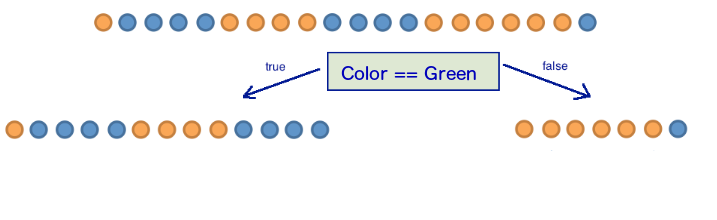
\includegraphics[width = \textwidth, keepaspectratio = true]{images/entropy}
\end{frame}

\begin{frame}{Критерий информационного выигрыша}
  \alert{Прирост информации} -- уменьшение энтропии.
  $$H = \sum\limits_{i=1}^{C} p_i \log_2 p_i$$\\
	$$IGain(U, x^j) = H(U) - \sum \limits_{v} \frac{\vert U_v\vert}{\vert U \vert} H(U_v) $$
  \bigbreak	
	$$v \in values(x^j) \qquad U_v = \{x \in U| x^j=v\}$$
\end{frame}

\begin{frame}{Плюсы}
	\begin{enumerate}[<+- |alert@+>] 
	\item[+] Интерпретируемость и простота классификации
	\item[+] Допустимы разнотипные данные и данные с пропусками
	\item[+] Не бывает отказов от классификации
	\item[+] Трудоёмкость линейна по длине выборки
	\end{enumerate}
\end{frame}

\begin{frame}{Минусы}
	\begin{enumerate} [<+- |alert@+>] 
	\item[--] Жадный ID3 сильно переобучается
	\item[--] Высокая чувствительность к шуму, к составу выборки, к критерию информативности
	\item[--] Чем дальше $v$ от корня, тем меньше надёжность выбора $\beta_v$ , $c_v$
	\end{enumerate}
\end{frame}

\begin{frame}{Переобучение}
  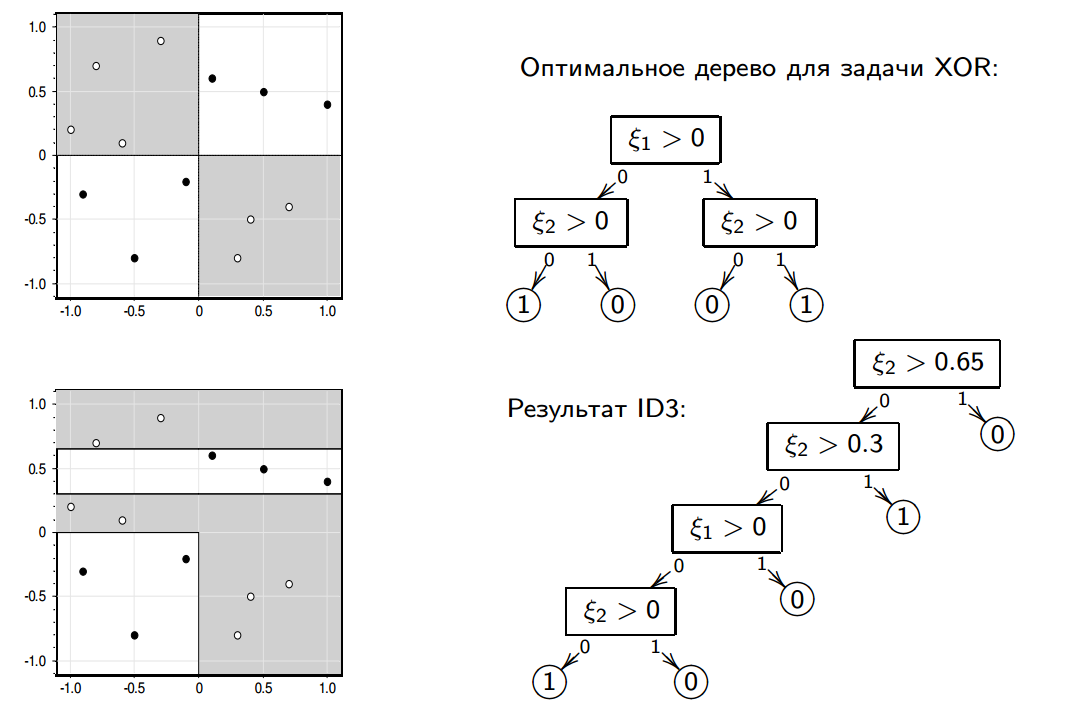
\includegraphics[height=190pt, keepaspectratio = true]{images/overfitting}   
\end{frame}

{\foot{pruning}
\begin{frame}{Подрезание дерева C4.5}
  $X^k$ -- независимая контрольная выборка, $k \approx 0.5l$\\
	Для всех $v \in V_{inner}$:\\
		\hspace{10mm} $U_v$ = подмножество объектов $X^k$, дошедших до $v$\\
		\hspace{10mm} Если $U_v = \oslash$:\\
		  \hspace{20mm} Вернуть новый лист $v$, $c_v$ = Majority(U)\\
		\hspace{10mm} Вычислить число ошибок четырьмя способами:\\
			\hspace{20mm} $r(v)$ -- поддеревом, растущим из вершины $v$\\
			\hspace{20mm} $r_L(v)$ -- левой дочерней вершины $L_v$\\
			\hspace{20mm} $r_R(v)$ -- правой дочерней вершины $R_v$\\
			\hspace{20mm} $r_c(v)$ -- к классу $c \in Y$\\
		\hspace{10mm} В зависимости от того, какое из них минимально:\\
			\hspace{20mm} Сохранить поддерево $v$\\
			\hspace{20mm} Заменить поддерево $v$ поддеревом $L_v$\\
			\hspace{20mm} Заменить поддерево $v$ поддеревом $R_v$\\
			\hspace{20mm} Заменить $v$ листом $c_v = \min\limits_{c \in Y} r_c(v)$\\
\end{frame}
}

{\foot{Oblivious Decision Trees}
\begin{frame}{Небрежные решающие деревья}
  \alert{Идея}: Сделаем дерево сбалансированным. Для этого нужно для всех узлов одного уровня использовать одинаковое условие ветвления.
  \pause
  \bigbreak
  
\includegraphics[width = \textwidth, keepaspectratio = true]{images/decisiontree}
\end{frame}
}

\begin{frame}{Композиция деревьев}
  \alert{Идея}: Можно использовать результаты нескольких	алгоритмов, а не одного.
\end{frame}

\begin{frame}{Random forest}
	Голосование деревьев классификации, $Y = \left\{ -1, +1 \right\}$\\
	$a(t) = Majority(b_t(x))$%\sign \frac{1}{T} \sum\limits_{t=1}^T b_t(x)$\\
	\begin{enumerate}[--]
  	  \item Каждое дерево $b_t(x)$ обучается по случайной выборке с повторениями
	  \item В каждой вершине предикат выбирается из случайного подмножества $\sqrt{n}$ предикатов
	\end{enumerate}
\end{frame}

\begin{frame}[standout]
  Вопросы?
\end{frame}

\appendix

\begin{frame}\frametitle{Что почитать по этой лекции}
  \begin{itemize}
    \item G. James, D. Witten, T. Hastie, R. Tibshirani "An Introduction to Statistical Learning" Chapter 8
    \item \href{http://www.machinelearning.ru/wiki/images/3/3e/Voron-ML-Logic.pdf}{Воронцов "Логические алгоритмы классификации"}
  \end{itemize}
\end{frame}

\begin{frame}{На следующей лекции}
  	\begin{enumerate} [--]
		\item Байесовские методы классификации
		\item Вероятностная постановка задачи
		\item Оптимальный Байесов классификатор
		\item Наивность
		\item Максимальное правдоподобие
		\item Разные распределения
	\end{enumerate}
\end{frame}


\end{document}